\usepackage{xspace}

\newcommand*{\plogo}{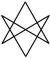
\includegraphics[scale=.5]{./include/pics/uch_small}} 

\makeatletter
\newcommand\mytitle[1]{\renewcommand\@mytitle{#1}}
\newcommand\@mytitle{}
\makeatother

\makeatletter
\newcommand\mysubtitle[1]{\renewcommand\@mysubtitle{#1}}
\newcommand\@mysubtitle{}
\makeatother

\makeatletter
\newcommand\myversion[1]{\renewcommand\@myversion{#1}}
\newcommand\@myversion{}
\makeatother


\newcommand{\myauthor}[1]{\author{#1}}


%-------------------------------------------------------------------------------
%	TITLE PAGE
%-------------------------------------------------------------------------------

\makeatletter
\newcommand*{\titleGP}{\begingroup 
\centering
\vspace*{\baselineskip} 

\rule{\textwidth}{1.6pt}\vspace*{-\baselineskip}\vspace*{2pt} 
\rule{\textwidth}{0.4pt}\\[\baselineskip]

{\Huge \scshape\@mytitle \\[0.2\baselineskip] }

\rule{\textwidth}{0.4pt}\vspace*{-\baselineskip}\vspace{3.2pt} 
\rule{\textwidth}{1.6pt}\\[\baselineskip] 

\scshape % Small caps
\@mysubtitle \\[\baselineskip] % Tagline(s) or further 
\today\par % Location and year

\vspace*{2\baselineskip} % Whitespace between location/year and editors

{\large \@author \par}

\vfill % Whitespace between editor names and publisher logo

\plogo \\[0.3\baselineskip] % Publisher logo
{Version \@myversion} \\[0.3\baselineskip] % Year published
% {\large THE PUBLISHER}\par % Publisher

\endgroup}
\makeatother


\newcommand{\makefirstfew}{%
\prebodyheadfoot
\restoregeometry

  
\titleGP
\newpage

% \input{./include/00-acknowledgement}
\vfill
\null
\vfill
\copyright\ 2014 Drew Schmidt and Christian Heckendorf.

Permission is granted to make and distribute verbatim copies of
this vignette and its source provided the copyright notice and
this permission notice are preserved on all copies.

This manual may be incorrect or out-of-date.  The authors assume
no responsibility for errors or omissions, or for damages resulting
from the use of the information contained herein.

Cover art is \textit{Hydra}, uploaded to \url{openclipart.org} by Tavin.

This publication was typeset using \LaTeX.

\newpage
\pagenumbering{roman}
\tableofcontents
\newpage


\pagenumbering{arabic}
\setcounter{page}{1}


\bodyheadfoot
\pagenumbering{arabic}
\setcounter{page}{1}
\pagestyle{fancy}
}

%%%%%%%%%%%%%%%%%%%%%%%%%%%%%%%%%%%%%%%%%%%%%%%%%%%%%%%%%%%%%%%%%%%%%%%%%%%%%%%%
%%%%% definitions
%%%%%%%%%%%%%%%%%%%%%%%%%%%%%%%%%%%%%%%%%%%%%%%%%%%%%%%%%%%%%%%%%%%%%%%%%%%%%%%%

\makeatletter
\newcommand\code{\bgroup\@makeother\_\@makeother\~\@makeother\$\@codex}
\def\@codex#1{{\normalfont\ttfamily\hyphenchar\font=-1 #1}\egroup}
\makeatother
%%\let\code=\texttt
\let\proglang=\textsf

\newcommand{\pkg}[1]{{\fontseries{b}\selectfont #1}}




\newcommand\mnote[1]{\marginpar{\vspace*{-.8cm}#1}}

\newcommand\easy{\mnote{\LARGE\color{green} \textbf{Easy}}}
\newcommand\medium{\mnote{\LARGE\color{yellow2} \textbf{Medium}}}
\newcommand\hard{\mnote{\LARGE\color{red} \textbf{Hard}}}

%%%%%%%%%%%%%%%%%%%%%%%%%%%%%%%%%%%%%%%%%%%%%%%%%%%%%%%%%%%%%%%%%%%%%%%%%%%%%%%%%%%%%%%%%%%%%%%%%%%%%%%%%%%%%%%%%%%%%%%%%%%%%%
%%%%% paragraph spacing
%%%%%%%%%%%%%%%%%%%%%%%%%%%%%%%%%%%%%%%%%%%%%%%%%%%%%%%%%%%%%%%%%%%%%%%%%%%%%%%%%%%%%%%%%%%%%%%%%%%%%%%%%%%%%%%%%%%%%%%%%%%%%%
\usepackage{parskip}
\setlength{\parskip}{.3cm}

%%%%%%%%%%%%%%%%%%%%%%%%%%%%%%%%%%%%%%%%%%%%%%%%%%%%%%%%%%%%%%%%%%%%%%%%%%%%%%%%%%%%%%%%%%%%%%%%%%%%%%%%%%%%%%%%%%%%%%%%%%%%%%
%%%%% colors
%%%%%%%%%%%%%%%%%%%%%%%%%%%%%%%%%%%%%%%%%%%%%%%%%%%%%%%%%%%%%%%%%%%%%%%%%%%%%%%%%%%%%%%%%%%%%%%%%%%%%%%%%%%%%%%%%%%%%%%%%%%%%%
\usepackage{xcolor}

\definecolor{yellow2}{rgb}{1, .7, 0}

\definecolor{mygreen}{RGB}{0,150,0}

\definecolor{gray}{rgb}{.6,.6,.6}
\definecolor{dkgray}{rgb}{.3,.3,.3}
\definecolor{orange}{rgb}{1,0.5,0}
\definecolor{grayish}{rgb}{.92, .92, .92}
\definecolor{grayishish}{HTML}{BDDDFF}

\definecolor{dkgreen}{rgb}{0,0.6,0}
\definecolor{mauve}{rgb}{0.58,0,0.82}

\definecolor{p0}{RGB}{150,0,0}
\definecolor{p1}{RGB}{0,150,0}
\definecolor{p2}{RGB}{0,0,150}
\definecolor{p3}{RGB}{150,75,0}



\definecolor{g11}{rgb}{0, 0, 1}
\definecolor{g12}{rgb}{0, .4, 1}
\definecolor{g13}{rgb}{0, .8, 1}

\definecolor{g21}{rgb}{0, .5, .3}
\definecolor{g22}{rgb}{.4, .5, .3}
\definecolor{g23}{rgb}{.8, .5, .3}


%%%%%%%%%%%%%%%%%%%%%%%%%%%%%%%%%%%%%%%%%%%%%%%%%%%%%%%%%%%%%%%%%%%%%%%%%%%%%%%%%%%%%%%%%%%%%%%%%%%%%%%%%%%%%%%%%%%%%%%%%%%%%%
%%%%% lstlisting
%%%%%%%%%%%%%%%%%%%%%%%%%%%%%%%%%%%%%%%%%%%%%%%%%%%%%%%%%%%%%%%%%%%%%%%%%%%%%%%%%%%%%%%%%%%%%%%%%%%%%%%%%%%%%%%%%%%%%%%%%%%%%%
\usepackage{listings}

\definecolor{rcomment}{rgb}{0.0,0.4,0.0}

\lstdefinelanguage{rr}{ 
	language=R,
	basicstyle=\ttfamily\color{black},
	backgroundcolor=\color{grayish},
	frame=single,
	breaklines=true,
	keywordstyle=\color{blue},
	commentstyle=\color{rcomment},
	stringstyle=\color{mauve},
	numbers=left,
	numberstyle=\tiny\color{dkgray},
	stepnumber=1,
	numbersep=8pt,
	showspaces=false,
	showstringspaces=false,
	showtabs=false,
	rulecolor=\color{gray},
	tabsize=4,
	captionpos=t,
	morekeywords={install_github, github, ngram, readLines, concatenate}
}


\lstdefinelanguage{inteRactive}{ 
        basicstyle=\ttfamily\color{black},
        backgroundcolor=\color{white},
        frame=single,
        breaklines=true,
        commentstyle=\color{blue},
        numbers=left,
        numberstyle=\tiny\color{dkgray},
        stepnumber=1,
        numbersep=8pt,
        showspaces=false,
        showstringspaces=false,
        showtabs=false,
        rulecolor=\color{gray},
        tabsize=4,
        morecomment=[l]{>}
}


\lstset{
	numbers=none,
	numberstyle=\footnotesize\ttfamily,
	frame=single,
	frameround=tttt,
	showspaces=false,
	showstringspaces=false,
	breaklines=true,
	breakatwhitespace=true,
	basicstyle=\small\ttfamily
}
  
%\lstset{literate={<-}{{$\leftarrow$}}1}
\makeatletter
\let\Code\@undefined
\let\CodeInput\@undefined
\let\CodeOutput\@undefined
\makeatother
\lstnewenvironment{Command}[1][title=Shell Command]{\lstset{#1}}{}
\lstnewenvironment{Code}[1][]{\lstset{#1}}{}
\lstnewenvironment{Output}[1][title=\ ]{\lstset{#1}}{}
\lstnewenvironment{CodeOutput}[1][title=R Output]{\lstset{#1}}{}
\lstnewenvironment{Error}[1][]{
  \lstset{title=Error Message,basicstyle=\small\ttfamily}\color{Red}}{}

  
  
\lstset{language=rr}

\lstdefinelanguage{rout}{ 
        language=R,
        basicstyle=\ttfamily\itshape\color{rcomment},
        backgroundcolor=\color{grayish},
        frame=single,
        breaklines=true,
        keywordstyle=\color{rcomment},
        commentstyle=\color{rcomment},
        stringstyle=\color{rcomment},
        numbers=left,
        numberstyle=\tiny\color{dkgray},
        stepnumber=1,
        numbersep=8pt,
        showspaces=false,
        showstringspaces=false,
        showtabs=false,
        rulecolor=\color{gray},
        tabsize=4,
        captionpos=t
}

\makeatletter
\newcommand\langname@rout{}
\def\langname@rout{rout}
\newcommand\prompt@rout{\#\#\ }
\newcommand\addedToEveryPar@rout{}
\lst@AddToHook{EveryPar}{\addedToEveryPar@rout}
\lst@AddToHook{PreInit}{%
  \ifx\lst@language\langname@rout%
    \let\addedToEveryPar@rout\prompt@rout%
  \fi
}
\makeatother


\lstdefinestyle{Rstyle}{language=rr}
\lstdefinestyle{Routstyle}{language=rout}



%%%%%%%%%%%%%%%%%%%%%%%%%%%%%%%%%%%%%%%%%%%%%%%%%%%%%%%%%%%%%%%%%%%%%%%%%%%%%%%%%%%%%%%%%%%%%%%%%%%%%%%%%%%%%%%%%%%%%%%%%%%%%%
%%%%% Headers/footers
%%%%%%%%%%%%%%%%%%%%%%%%%%%%%%%%%%%%%%%%%%%%%%%%%%%%%%%%%%%%%%%%%%%%%%%%%%%%%%%%%%%%%%%%%%%%%%%%%%%%%%%%%%%%%%%%%%%%%%%%%%%%%%

\usepackage{./include/lastpage}
\usepackage{fancyhdr}

\pagestyle{fancy}

\newcommand{\prebodyheadfoot}{
  \fancyhf{} % clear all header and footer fields
  \fancyfoot{}
  \renewcommand{\headrulewidth}{0pt}
  \renewcommand{\footrulewidth}{0pt}
  
  % redefinition of the plain style:
  \fancypagestyle{plain}{%
  \fancyhf{} % clear all header and footer fields
  \renewcommand{\headrulewidth}{0pt}
  \renewcommand{\footrulewidth}{0pt}}
}

\newcommand{\bodyheadfoot}{
  \fancyhf{} % clear all header and footer fields
% \fancyhead[L]{\slshape \rightmark}
  \fancyhead[L]{\slshape \leftmark}
  \fancyhead[R]{ \thepage\ of\ \pageref{LastPage}}
  \renewcommand{\headrulewidth}{1pt}
  \renewcommand{\footrulewidth}{0pt}
  
  % redefinition of the plain style:
  \fancypagestyle{plain}{%
  \fancyhf{} % clear all header and footer fields
  \renewcommand{\headrulewidth}{0pt}
  \renewcommand{\footrulewidth}{0pt}}
}

%%%%%%%%%%%%%%%%%%%%%%%%%%%%%%%%%%%%%%%%%%%%%%%%%%%%%%%%%%%%%%%%%%%%%%%%%%%%%%%%%%%%%%%%%%%%%%%%%%%%%%%%%%%%%%%%%%%%%%%%%%%%%%
%%%%% misc.
%%%%%%%%%%%%%%%%%%%%%%%%%%%%%%%%%%%%%%%%%%%%%%%%%%%%%%%%%%%%%%%%%%%%%%%%%%%%%%%%%%%%%%%%%%%%%%%%%%%%%%%%%%%%%%%%%%%%%%%%%%%%%%

\usepackage{xspace}
\newcommand{\R}{\proglang{R}\xspace}
\newcommand{\C}{\proglang{C}\xspace}
\newcommand{\CXX}{\proglang{C$++$}\xspace}

\newcommand{\PAPI}{\pkg{PAPI}\xspace}

\definecolor{pbdgrn}{HTML}{005700}
\definecolor{pbdrd}{HTML}{ab0000}
\definecolor{pbdylw}{HTML}{ab7e00}
\definecolor{pbdblu}{HTML}{2b74ec}
\newcommand{\pbdR}{\textbf{\color{pbdgrn}{p}\color{pbdrd}{b}\color{pbdylw}{d}\color{pbdblu}{R}\xspace}}

% \usepackage{url}
\usepackage{multirow}
\usepackage{amsmath}
\usepackage{amsthm}
\usepackage{amssymb}
% \usepackage{subfig}
\usepackage{graphicx}


\usepackage{hyperref}

\hypersetup{
    pdfnewwindow=true,
    colorlinks=true,
    linkcolor=blue,
    citecolor=blue,
    filecolor=magenta,
    urlcolor=blue
}

\newcommand{\secref}[1]{\hyperref[#1]{Section~\ref*{#1}}}

\newcommand{\twiddle}[1]{\hspace{.05cm}$\sim$~\hspace{-.1cm}#1\hspace{-.1cm}~$\sim$\hspace{.05cm}}





%%%%%%%%%%%%%%%%%%%%%%%%%%%%%%%%%%%%%%%%%%%%%%%%%%%%%%%%%%%%%%%%%%%%%%%%%%%%%%%%%%%%%%%%%%%%%%%%%%%%%%%%%%%%%%%%%%%%%%%%%%%%%%
%%%%% Bibliography
%%%%%%%%%%%%%%%%%%%%%%%%%%%%%%%%%%%%%%%%%%%%%%%%%%%%%%%%%%%%%%%%%%%%%%%%%%%%%%%%%%%%%%%%%%%%%%%%%%%%%%%%%%%%%%%%%%%%%%%%%%%%%%

\usepackage[nottoc,notlof,notlot]{tocbibind}
\usepackage[authoryear,round]{natbib}
\usepackage{multirow}
